\section{Auswertung}
\label{sec:Auswertung}

\subsection{Eichung des Magnetfeldes}

Zunächst wird eine Eichung des Magnetfeldes vorgenommen. Zu diesem Zweck werden die Stromstärken zwischen 0 bis 5 Ampere eingestellt 
und das entstehende Magnetfeld mittels einer Hallsonde gemessen. Die aufgenommenen Messwerte sind in Tabelle --- zu sehen. 

\begin{table}[H]
    \centering
    \caption{Messwerte für die Eichung des Magnetfeldes.}
    \label{tab:mess1}
    \sisetup{table-format=2.1}
    \begin{tabular}{c c}
    \toprule
    $I \;/\; \si{\ampere}$ & $B \;/\; \si{\milli\tesla}$ \\
    \midrule
        0 & 0\\
        0,51 & 45\\
        1,01 & 90\\
        1,53 & 139\\
        2,00 & 182\\
        2,52 & 231\\
        3,02 & 276\\
        3,50 & 318\\
        4,03 & 363\\
        4,51 & 402\\
        4,99 & 435\\
    \bottomrule
    \end{tabular}
  \end{table}
  
  Diese Messwerte sind in Abbildung \ref{fig:plot1} graphisch dargestellt. 
  
\begin{figure}
    \centering
    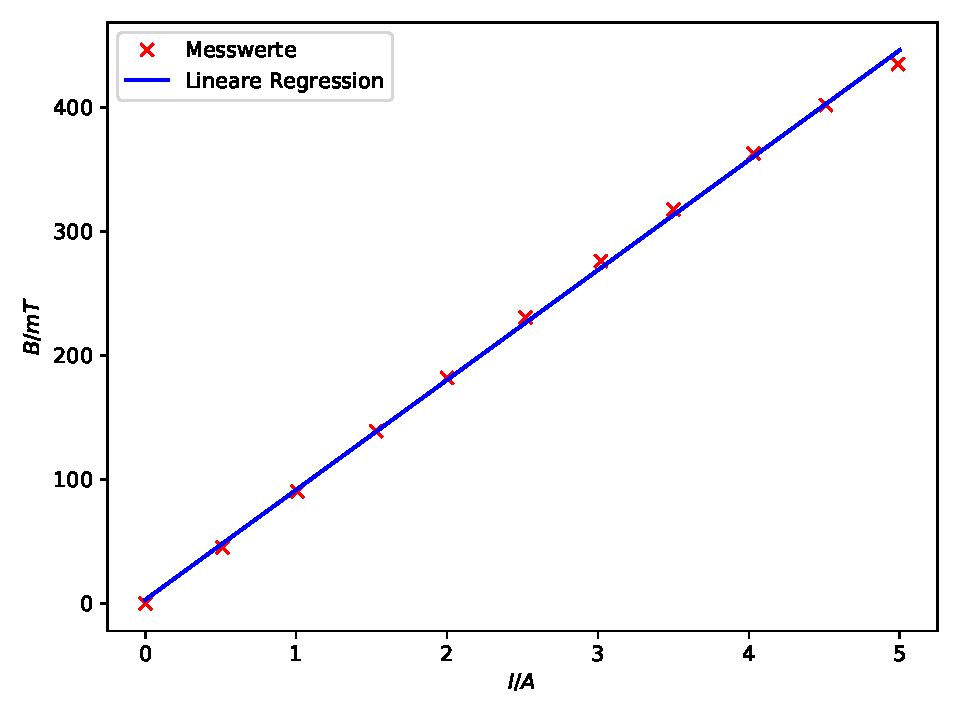
\includegraphics[scale=0.7]{content/plot1.pdf}
    \vspace{-10pt}
    \caption{Lineare Regression des Magnetfeldes $B$ in Abhängigkeit der angelegten Stromstärke $I$.}
    \label{fig:plot1}
\end{figure}

Dabei wird eine linear Regression mit 

\begin{equation*}
    B(I) = a\cdot I + b
\end{equation*}

durchgeführt. Die Parameter ergeben sich dabei zu 

\begin{align*}
    a &= \SI{88.68+-0.93}{\milli\tesla\per\ampere}, \\
    b &= \SI{2.88+-2.77}{\milli\tesla}.
\end{align*}

\subsection{Untersuchung der roten Spektrallinie}

Um den Lande-Faktor des linear polarisierten Lichtes der roten Cadmium-Linie zu bestimmen wird das Interferenzmuster aufgenommen. Dieses
ist in Abbidlung \ref{fig:rot} zu sehen. 

\begin{figure}
    \centering
    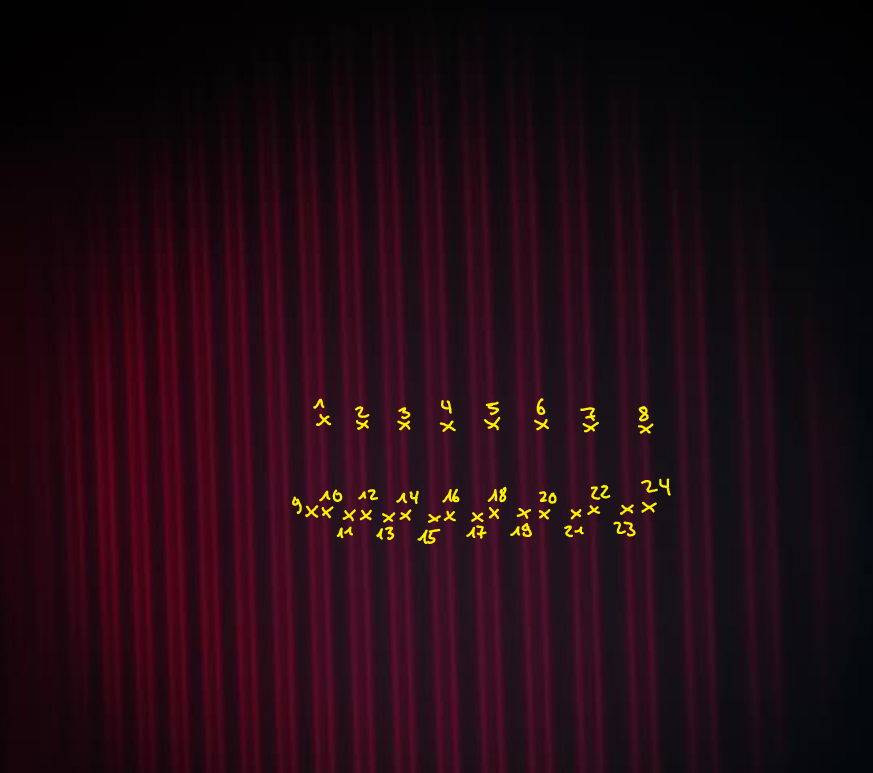
\includegraphics[scale=0.35]{content/rot.png}
    \vspace{-10pt}
    \caption{Interferenzmuster der roten Cadmium-Linie mit eingeschaltetem Magnetfeld.}
    \label{fig:rot}
\end{figure}

Die Spule wird dabei mit $\SI{5}{\ampere}$ betrieben. Die eingezeichneten gelben Punkte 1 bis 8 werden zur Bestimmung der Abstände
zwischen den Linien ohne Magnetfeld verwendet. Ihre Positionswerte sind in Tabelle \ref{tab:mess2} aufgeführt. 

\begin{table}[H]
    \centering
    \caption{Messwerte zur Abstandsbestimmung der roten Cadmium-Linie ohne Magnetfeld.}
    \label{tab:mess2}
    \sisetup{table-format=2.1}
    \begin{tabular}{c c}
    \toprule
    $\text{Punkt}$ & $x \;/\; \text{px}$ \\
    \midrule
        1 & 1574\\
        2 & 1706\\
        3 & 1846\\
        4 & 1990\\
        5 & 2142\\
        6 & 2300\\
        7 & 2474\\
        8 & 2652\\
    \bottomrule
    \end{tabular}
\end{table}

Daraus ergibt sich 

\begin{equation*}
    \symup{\Delta} s_\text{rot} = \num{154.0+-15.9}\quad\text{px}.
\end{equation*}

Zur Bestimmung der Linienauftrennung durch das Magnetfeld werden die Punkte 9 bis 24 genutzt. Die Messwerte ihrer Position befinden sich in 
Tabelle \ref{tab:mess3}. 

\begin{table}[H]
    \centering
    \caption{Messwerte zur Abstandsbestimmung der roten Cadmium-Linie mit Magnetfeld.}
    \label{tab:mess3}
    \sisetup{table-format=2.1}
    \begin{tabular}{c c}
    \toprule
    $\text{Punkt}$ & $x \;/\; \text{px}$ \\
    \midrule
        9 & 1536\\
        10 & 1582\\
        11 & 1664\\
        12 & 1716\\
        13 & 1804\\
        14 & 1854\\
        15 & 1946\\
        16 & 1998\\
        17 & 2094\\
        18 & 2146\\
        19 & 2248\\
        20 & 2306\\
        21 & 2412\\
        22 & 2476\\
        23 & 2588\\
        24 & 2658\\
    \bottomrule
    \end{tabular}
\end{table}

Mit diesen Messdaten folgt

\begin{equation*}
    \delta s_\text{rot} = \num{55.5+-7.5}\quad \text{px}.    
\end{equation*}

Werden diese Werte in 

\begin{equation*}
    \delta \lambda = \frac{\delta s}{\Delta s}\frac{\Delta \lambda}{2}
\end{equation*}

eingesetzt, ergibt sich 

\begin{equation*}
    \delta \lambda = \SI{8.8+-1.5}{\pico\metre}.
\end{equation*}

Nun kann mittels 

\begin{equation}
    g = \frac{hc\cdot\delta\lambda}{\lambda^2\mu_\text{B}B}
\end{equation}

der Lande-Faktor zu 

\begin{equation*}
    g = \num{1.04+-0.18}
\end{equation*}

bestimmt werden. 

\subsection{Untersuchung von sigma-polarisiertem Licht der blauen Cadmium-Linie}

Zunächst werden erneut die Abstände der Interferenzlinien der blauen Cadmium-Linie ohne Magnetfeld bestimmt. Das
aufgenommene Interferenzbild ist in Abbildung \ref{fig:blau_ohne} zu sehen. 

\begin{figure}
    \centering
    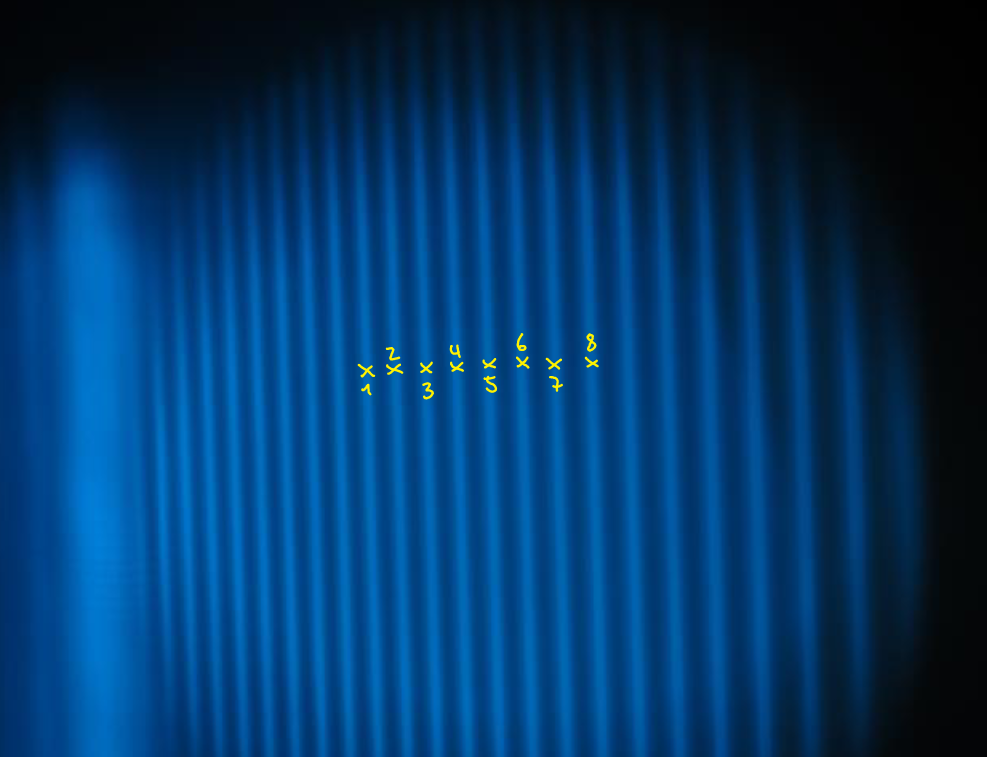
\includegraphics[scale=0.35]{content/blau_ohne.png}
    \vspace{-10pt}
    \caption{Interferenzmuster der blauen Cadmium-Linie ohne Magnetfeld.}
    \label{fig:blau_ohne}
\end{figure}

Die Positionen der Punkte sind in Tabelle \ref{tab:mess4} aufgeführt.

\begin{table}[H]
    \centering
    \caption{Messwerte zur Abstandsbestimmung der roten Cadmium-Linie ohne Magnetfeld.}
    \label{tab:mess4}
    \sisetup{table-format=2.1}
    \begin{tabular}{c c}
    \toprule
    $\text{Punkt}$ & $x \;/\; \text{px}$ \\
    \midrule
        1 & 1510\\
        2 & 1606\\
        3 & 1706\\
        4 & 1810\\
        5 & 1914\\
        6 & 2024\\
        7 & 2140\\
        8 & 2260\\
    \bottomrule
    \end{tabular}
\end{table}

Damit ergibt sich 

\begin{equation*}
    \symup{\Delta} s_\text{blau} = \num{107.14+-7.99} \quad \text{px}.
\end{equation*}

Nun wird ein Magnetfeld von $B = \SI{318}{\milli\tesla}$ angelegt und das Interferenzbild fotografiert. Dieses 
ist in Abbildung \ref{fig:blau_mit} zu sehen. 

\begin{figure}
    \centering
    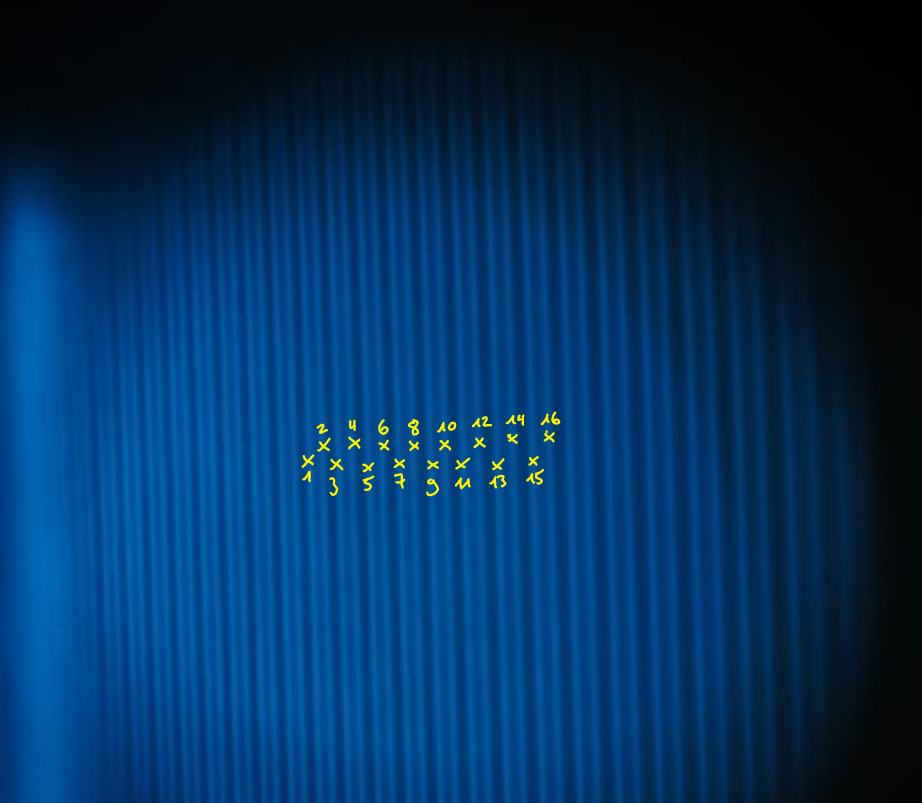
\includegraphics[scale=0.35]{content/blau_mit.png}
    \vspace{-10pt}
    \caption{Interferenzmuster der blauen Cadmium-Linie mit Magnetfeld.}
    \label{fig:blau_mit}
\end{figure}

Die Positionen der Punkte ergeben sich zu den Messwerten in Tabelle \ref{tab:mess5}. 

\begin{table}[H]
    \centering
    \caption{Messwerte zur Abstandsbestimmung der roten Cadmium-Linie mit Magnetfeld.}
    \label{tab:mess5}
    \sisetup{table-format=2.1}
    \begin{tabular}{c c}
    \toprule
    $\text{Punkt}$ & $x \;/\; \text{px}$ \\
    \midrule
        1 & 1488\\
        2 & 1538\\
        3 & 1588\\
        4 & 1636\\
        5 & 1690\\
        6 & 1736\\
        7 & 1792\\
        8 & 1840\\
        9 & 1896\\
        10 & 1950\\
        11 & 2004\\
        12 & 2060\\
        13 & 2122\\
        14 & 2172\\
        15 & 2242\\
        16 & 2294\\
    \bottomrule
    \end{tabular}
\end{table}

Mit diesen Werten folgt 

\begin{equation*}
    \delta s_\text{blau} = \num{50.5+-3.12}\quad \text{px}.
\end{equation*}

Damit lässt sich erneut $\delta \lambda$ folgern zu 

\begin{equation*}
    \delta \lambda = \SI{6.4+-0.6}{\pico\metre}
\end{equation*}

und damit der Lande-Faktor bestimmen zu 

\begin{equation*}
    g = \num{1.85+-0.18}.
\end{equation*}

\subsection{Untersuchung von pi-polarisiertem Licht der blauen Cadmium-Linie}



Um den Lande-Faktor des linear polarisierten Lichtes der blauen Cadmium-Linie zu bestimmen wird das Interferenzmuster aufgenommen. Dieses
ist in Abbidlung \ref{fig:blaupi} zu sehen. 

\begin{figure}
    \centering
    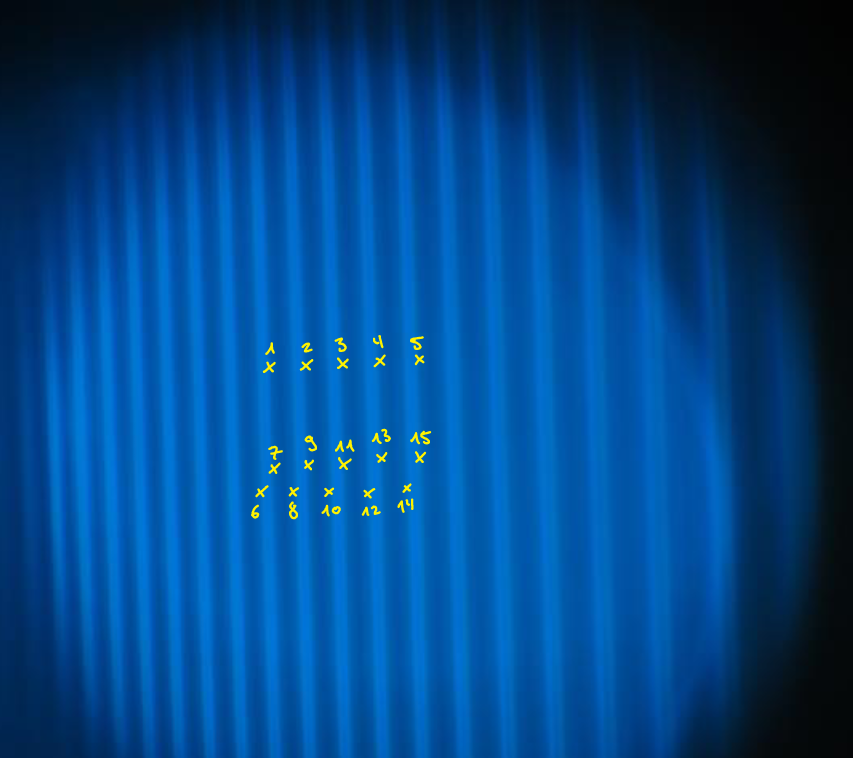
\includegraphics[scale=0.35]{content/blau_pi.png}
    \vspace{-10pt}
    \caption{Interferenzmuster der blauen Cadmium-Linie mit eingeschaltetem Magnetfeld.}
    \label{fig:blaupi}
\end{figure}

Die Spule wird dabei mit $\SI{5}{\ampere}$ betrieben. Die eingezeichneten gelben Punkte 1 bis 5 werden zur Bestimmung der Abstände
zwischen den Linien ohne Magnetfeld verwendet. Ihre Positionswerte sind in Tabelle \ref{tab:mess6} aufgeführt. 

\begin{table}[H]
    \centering
    \caption{Messwerte zur Abstandsbestimmung der blauen Cadmium-Linie ohne Magnetfeld.}
    \label{tab:mess6}
    \sisetup{table-format=2.1}
    \begin{tabular}{c c}
    \toprule
    $\text{Punkt}$ & $x \;/\; \text{px}$ \\
    \midrule
        1 & 932\\
        2 & 1048\\
        3 & 1164\\
        4 & 1290\\
        5 & 1426\\
    \bottomrule
    \end{tabular}
\end{table}

Daraus ergibt sich 

\begin{equation*}
    \symup{\Delta} s_\text{rot} = \num{123.5+-8.29}\quad\text{px}.
\end{equation*}

Zur Bestimmung der Linienauftrennung durch das Magnetfeld werden die Punkte 6 bis 15 genutzt. Die Messwerte ihrer Position befinden sich in 
Tabelle \ref{tab:mess7}. 

\begin{table}[H]
    \centering
    \caption{Messwerte zur Abstandsbestimmung der blauen Cadmium-Linie mit Magnetfeld.}
    \label{tab:mess7}
    \sisetup{table-format=2.1}
    \begin{tabular}{c c}
    \toprule
    $\text{Punkt}$ & $x \;/\; \text{px}$ \\
    \midrule
        6 & 892\\
        7 & 932\\
        8 & 1008\\
        9 & 1048\\
        10 & 1126\\
        11 & 1164\\
        12 & 1254\\
        13 & 1290\\
        14 & 1384\\
        15 & 1426\\
    \bottomrule
    \end{tabular}
\end{table}

Mit diesen Messdaten folgt

\begin{equation*}
    \delta s_\text{rot} = \num{39.2+-2.04}\quad \text{px}.    
\end{equation*}

Werden diese Werte in 

\begin{equation*}
    \delta \lambda = \frac{\delta s}{\Delta s}\frac{\Delta \lambda}{2}
\end{equation*}

eingesetzt, ergibt sich 

\begin{equation*}
    \delta \lambda = \SI{4.3+-0.4}{\pico\metre}.
\end{equation*}

Nun kann mittels 

\begin{equation}
    g = \frac{hc\cdot\delta\lambda}{\lambda^2\mu_\text{B}B}
\end{equation}

der Lande-Faktor zu 

\begin{equation*}
    g = \num{0.91+-0.08}
\end{equation*}

bestimmt werden. 